

% Gradient Info
  
\tikzset {_ltuftconh/.code = {\pgfsetadditionalshadetransform{ \pgftransformshift{\pgfpoint{0 bp } { -1.5 bp }  }  \pgftransformrotate{-90 }  \pgftransformscale{2 }  }}}
\pgfdeclarehorizontalshading{_116066l99}{150bp}{rgb(0bp)=(1,1,1);
rgb(37.5bp)=(1,1,1);
rgb(62.5bp)=(0,0,0);
rgb(100bp)=(0,0,0)}
\tikzset{_7hyra6oev/.code = {\pgfsetadditionalshadetransform{\pgftransformshift{\pgfpoint{0 bp } { -1.5 bp }  }  \pgftransformrotate{-90 }  \pgftransformscale{2 } }}}
\pgfdeclarehorizontalshading{_tamkewics} {150bp} {color(0bp)=(transparent!0);
color(37.5bp)=(transparent!0);
color(62.5bp)=(transparent!10);
color(100bp)=(transparent!10) } 
\pgfdeclarefading{_2goarmiec}{\tikz \fill[shading=_tamkewics,_7hyra6oev] (0,0) rectangle (50bp,50bp); } 

% Gradient Info
  
\tikzset {_tmoau9aoq/.code = {\pgfsetadditionalshadetransform{ \pgftransformshift{\pgfpoint{0 bp } { 0 bp }  }  \pgftransformrotate{-90 }  \pgftransformscale{2 }  }}}
\pgfdeclarehorizontalshading{_w69zgx8r6}{150bp}{rgb(0bp)=(1,0,0);
rgb(41.607142857142854bp)=(1,0,0);
rgb(49.01785714285714bp)=(1,0,0);
rgb(58.48214285714286bp)=(0.29,0.56,0.89);
rgb(100bp)=(0.29,0.56,0.89)}
\tikzset{every picture/.style={line width=0.75pt}} %set default line width to 0.75pt        

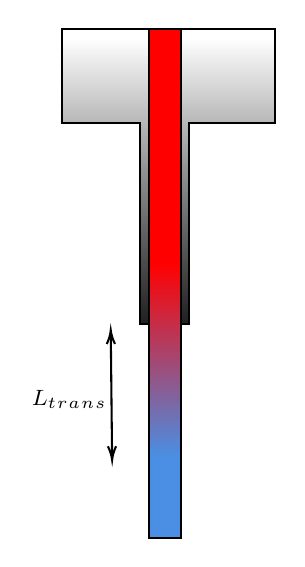
\begin{tikzpicture}[x=0.75pt,y=0.75pt,yscale=-1,xscale=1]
%uncomment if require: \path (0,300); %set diagram left start at 0, and has height of 300

%Shape: Path Data [id:dp4697754887314718] 
\path  [shading=_116066l99,_ltuftconh,path fading= _2goarmiec ,fading transform={xshift=2}] (308.72,191.41) -- (285.13,191.41) -- (285.13,94.42) -- (247.68,94.42) -- (247.68,49) -- (350.33,49) -- (350.33,94.42) -- (308.72,94.42) -- (308.72,191.41) -- cycle ; % for fading 
 \draw   (308.72,191.41) -- (285.13,191.41) -- (285.13,94.42) -- (247.68,94.42) -- (247.68,49) -- (350.33,49) -- (350.33,94.42) -- (308.72,94.42) -- (308.72,191.41) -- cycle ; % for border 

%Shape: Rectangle [id:dp38851785666306216] 
\path  [shading=_w69zgx8r6,_tmoau9aoq] (304.89,294.2) -- (304.89,49) -- (289.37,49) -- (289.37,294.2) -- cycle ; % for fading 
 \draw   (304.89,294.2) -- (304.89,49) -- (289.37,49) -- (289.37,294.2) -- cycle ; % for border 

%Straight Lines [id:da23182528010896997] 
\draw    (271.05,196.32) -- (271.67,254.74) ;
\draw [shift={(271.7,256.74)}, rotate = 269.39] [color={rgb, 255:red, 0; green, 0; blue, 0 }  ][line width=0.75]    (6.56,-1.97) .. controls (4.17,-0.84) and (1.99,-0.18) .. (0,0) .. controls (1.99,0.18) and (4.17,0.84) .. (6.56,1.97)   ;
\draw [shift={(271.03,194.32)}, rotate = 89.39] [color={rgb, 255:red, 0; green, 0; blue, 0 }  ][line width=0.75]    (6.56,-1.97) .. controls (4.17,-0.84) and (1.99,-0.18) .. (0,0) .. controls (1.99,0.18) and (4.17,0.84) .. (6.56,1.97)   ;

% Text Node
\draw (231.51,221.9) node [anchor=north west][inner sep=0.75pt]  [font=\footnotesize] [align=left] {$\displaystyle L_{t}{}_{r}{}_{a}{}_{n}{}_{s}$};


\end{tikzpicture}
